\documentclass[]{article}
\usepackage[round]{natbib}

\usepackage[margin=1in]{geometry}
\usepackage{url}
\usepackage{authblk}
\usepackage{graphicx}
\usepackage{color}
\usepackage{xspace}
\usepackage{amsmath,amssymb}
\usepackage{longtable,booktabs,array}
\usepackage{calc} % for calculating minipage widths


% cross-reference with main text
\usepackage{xr}
\externaldocument{paper}


\begin{document}

\title{Supporting Information for\\
``A heterogeneous landscape of selection and epistasis in protein-coding genes''}
\author[]{Aaron P. Ragsdale}
\affil[1]{Department of Integrative Biology, University of Wisconsin, Madison, WI, USA}
\affil[*]{apragsdale@wisc.edu}
\date{\today}
\maketitle

\renewcommand{\thefigure}{S\arabic{figure}}
\renewcommand{\thetable}{S\arabic{table}}
\renewcommand{\theequation}{S\arabic{equation}}
\setcounter{figure}{0}
\setcounter{table}{0}
\setcounter{equation}{0}

\small
\tableofcontents
\normalsize
\newpage

\clearpage

\section{The diffusion equation and moment system for the two-locus sampling distribution}

The two-locus diffusion equation with additive selection was first described by
\citet{Kimura1955-qe} and studied extensively in the 1960s and 70s (e.g.,
\citet{Hill1966-gv,Ohta1969-ie}). The continuous distribution \(\psi(x_1, x_2,
x_3)\) of haplotype frequencies in a population, where \(x_1\) is the frequency
of \(AB\), \(x_2\) of \(Ab\), and \(x_3\) of \(aB\), is governed by the
multi-dimensional Fokker-Planck equation:
\begin{align} \label{eq:diffeq}
\frac{\partial \psi}{\partial \tau} = &
\frac{1}{2}\mathop{\sum\sum}_{1\leq i, j \leq 3}
\frac{\partial^2}{\partial x_i \partial x_j}
\left[\frac{x_i(\delta_{i=j}-x_j)\psi}{\nu(\tau)}\right] \\\nonumber
& -\frac{\rho}{2}\left(-\frac{\partial}{\partial x_1} D\psi
  + \frac{\partial}{\partial x_2} D\psi
  + \frac{\partial}{\partial x_3} D\psi\right) \\\nonumber
& - \frac{\gamma_A}{2}\left[
  \frac{\partial}{\partial x_1} x_1(1-x_1-x_2)\psi
  + \frac{\partial}{\partial x_2} x_2(1-x_1-x_2)\psi
  - \frac{\partial}{\partial x_3} x_3(x_1+x_2)\psi
  \right] \\\nonumber
& -\frac{\gamma_B}{2}\left[
  \frac{\partial}{\partial x_1} x_1(1-x_1-x_3)\psi
  - \frac{\partial}{\partial x_2} x_2(x_1+x_3)\psi
  + \frac{\partial}{\partial x_3} x_3(1-x_1-x_3)\psi
  \right].
\end{align}
\(D\) is the standard covariance measure of linkage disequilibrium, \[D=x_1 -
(x_1+x_2)(x_1+x_3) = x_1 x_4 - x_2 x_3,\] \(\gamma_A\) and \(\gamma_B\) are the
(additive) scaled selection coefficients at the left and right locus, and
\(\rho\) is the scaled recombination rate between the two loci. Time \(\tau\) is
measured in \(2N_e\) generations, and \(\nu(\tau)\) is the population size relative
to the ancestral size or some reference size at time \(\tau\).

Given a function \(\psi\) that solves Equation \ref{eq:diffeq}, the two-locus
sampling distribution for a sample size of \(n\) haploids can be found by
integrating \(\Psi\) against the multinomial sampling function, so that
\begin{align} \label{eq:multinomial}
\Psi_n(i, j, k) =
{n \choose{i, j, k, n-i-j-k}}
\mathop{\mathop{\int\int\int}_{x_1, x_2, x_3 \geq0}}_{x_1+x_2+x_3\leq1}
\psi(x_1, x_2, x_3) x_1^i x_2^j x_3^k (1-x_1-x_2-x_3)^{n-i-j-k}
dx_1 dx_2 dx_3.
\end{align}

In the method-of-moments approach, instead of solving the differential equation
for \(\psi\), we instead integrate both sides of the differential equation
against the multinomial sampling function for a given sampling configuration
\((i, j, k)\). On the left side, we get \(\partial_t \Psi_n(i, j, k)\), and on the
right we obtain, after some simple integration by parts and somewhat tedious
simplification, terms for drift, recombination, and selection that can be
written as sparse linear operators of \(\Psi_n\). Written compactly, this takes
the form
\begin{equation}
\partial_\tau \Psi_n =
\frac{1}{2\nu(\tau)}\mathcal{D}_{n}\Psi_n
+ \frac{\rho}{2}\mathcal{R}_{n}\Psi_n
+ \frac{\theta}{2}\mathcal{U}_{n}\Psi_n
+ \mathcal{S}_{n, \boldsymbol{\gamma}, \mathbf{h}}\Psi_n.
\end{equation}.

Alternatively, we arrive at this same linear system of equations by tracking
the expected sampling distribution over \(n\) lineages within the full population
and how that changes over time by drawing lineages from one generation to the
next in the style of \citet{Wright1931-wy}. Both \citet{Jouganous2017-pq}, for the
single-locus SFS, and \citet{Ragsdale2019-nt} drew this connection in detail, so I
refer readers to those previous papers for a fuller description of those
derivations and discussion. In the next section I simply repeat the results for
\(\mathcal{D}\), \(\mathcal{R}\), and \(\mathcal{U}\), briefly describe the moment
closure approximation (which is the same as presented in \citet{Ragsdale2019-nt}), and
then describe the selection operator \(\mathcal{S}\) for selection with
epistasis, both with and without dominance.

\subsection{Drift, mutation, recombination, and moment closure}\label{drift-mutation-recombination-and-moment-closure}

\subsubsection{Drift}\label{drift}

Drift for an entry \((i, j, k)\) depends only on \(\Psi_n\) and therefore closes.
The entries of \(\mathcal{D}\) are found by considering the possibility of a
coalescence event occurring within a given generation within \(n\) lineages in
the full population. If \(n \ll N\), we can safely assume that at most a single
such event occurs in any given generation.

\begin{align}
\mathcal{D}_{n}(i, j, k)\Psi_n =
& (i - 1) (n - i - j - k + 1) \Psi_n(i - 1, j, k) \\\nonumber
& + (i + 1) (n - i - j - k - 1) \Psi_n(i + 1, j, k) \\\nonumber
& + (i - 1) (k + 1) \Psi_n(i - 1, j, k + 1) \\\nonumber
& + (i + 1) (k - 1) \Psi_n(i + 1, j, k - 1) \\\nonumber
& + (i - 1) (j + 1) \Psi_n(i - 1, j + 1, k) \\\nonumber
& + (i + 1) (j - 1) \Psi_n(i + 1, j - 1, k) \\\nonumber
& + (j - 1) (n - i - j - k + 1) \Psi_n(i, j - 1, k) \\\nonumber
& + (j + 1) (n - i - j - k - 1) \Psi_n(i, j + 1, k) \\\nonumber
& + (j - 1) (k + 1) \Psi_n(i, j - 1, k + 1) \\\nonumber
& + (j + 1) (k - 1) \Psi_n(i, j + 1, k - 1) \\\nonumber
& + (k - 1) (n - i - j - k + 1) \Psi_n(i, j, k - 1) \\\nonumber
& + (k + 1) (n - i - j - k - 1) \Psi_n(i, j, k + 1) \\\nonumber
& - 2\left( i ( n - i - j - k) + i k + i j + j (n - i - j - k) + j k + k(n - i - j - k)\right)\Psi_n(i, j, k)
\end{align}

\subsubsection{Recombination}\label{recombination}

If a lineage in our sample of size \(n\) recombines in a given generation, which
occurs with probability \(nr\), we need to draw an extra lineage from the full
population for it to recombine with. This means we need \(\Psi_{n+1}\) in the
previous generation. After drawing that extra lineage, \(\Psi_n\) changes as we
draw one of the two recombinant types (each with probability \(1/2\)) instead of
the lineage that was chosen to recombine.

\begin{align}
\mathcal{R}_{n}(i, j, k)\Psi_n = &
\frac{(i + 1)(n - i - j - k + 1)}{n + 1}\Psi_{n+1}(i + 1, j - 1, k) \\\nonumber
& + \frac{(i + 1)(n - i - j - k + 1)}{n + 1}\Psi_{n+1}(i + 1, j, k - 1) \\\nonumber
& + \frac{(j + 1)(k + 1}{n + 1)}\Psi_{n+1}(i - 1, j + 1, k + 1) \\\nonumber
& + \frac{(j + 1)(k + 1}{n + 1)}\Psi_{n+1}(i, j + 1, k + 1) \\\nonumber
& - \frac{(i + 1)(n - i - j - k)}{n + 1}\Psi_{n+1}(i + 1, j, k) \\\nonumber
& - \frac{(j + 1) k}{n + 1}\Psi_{n+1}(i, j + 1, k) \\\nonumber
& - \frac{j (k + 1)}{n + 1}\Psi_{n+1}(i, j, k + 1) \\\nonumber
& - \frac{i (n - i - j - k + 1}{n + 1}\Psi_{n+1}(i, j, k)
\end{align}

\subsubsection{Mutation}\label{mutation}

We assume an infinite sites mutation (ISM) model where new mutations occur at
previously unmutated loci. In the two-locus ISM model, two-locus pairs of
variable loci arise when a mutation occurs at one locus when the other locus is
already variable. Thus, new mutations at the \(B/b\) locus occur against the
single-locus allele frequency distribution \(\Phi_{n,A}\), and new mutations at
the \(A/a\) locus occur against \(\Phi_{n, B}\), which are found via the single-locus
system from \citet{Jouganous2017-pq}.

\begin{align}
\mathcal{U}_{n}(i, j, k)\Psi_n = &
(j + 1)\frac{\theta_B}{2} \Phi_{n, A}(j+1) \delta_{i=1, k=0} \\\nonumber
& + (n - j)\frac{\theta_B}{2} \Phi_{n, A}(j) \delta_{i=0, k=1} \\\nonumber
& + (i + 1)\frac{\theta_A}{2} \Phi_{n, B}(i+1) \delta_{i=1, j=0} \\\nonumber
& + (n - i)\frac{\theta_A}{2} \Phi_{n, B}(i) \delta_{i=0, j=1} \\\nonumber
\end{align}

\subsubsection{Jackknife moment closure approximation}\label{jackknife-moment-closure-approximation}

We use a jackknife approximation to write the entries of \(\Psi_{n+1}\) and
\(\Psi_{n+2}\) as linear combinations of entries in \(\Psi_n\). The general
strategy is to assume the underlying continuous distribution \(\psi(x_1, x_2, x_3)\) can be approximated locally as a quadratic, and then use entries in
\(\Psi_n\) that are close in frequency to a given entry in \(\Psi_{n+l}\) to
estimate the coefficients of that quadratic using the multinomial sampling
formula. Then this quadratically local approximation to \(\psi\) can be used to
compute \(\Psi_{n+l}(i, j, k)\) using Eq. \eqref{eq:multinomial}. Readers should
refer to section S1.3.5 in the Supporting material for \citet{Ragsdale2019-nt} for
details.

\subsection{Selection}\label{selection}

First consider the case of no dominance, so that the haplotypes \(Ab\), \(aB\),
and \(AB\) have selection coefficients \(s_{Ab}\), \(s_{aB}\), and \(s_{AB}\),
respectively. Note that the case with \(s_{AB} = s_{Ab} + s_{aB}\) implies no
epistasis between the \(A/a\) and \(B/b\) loci. Here, we assume all selection
coefficients are negative. In a given generation, a selection event could
occur in which a haplotype is rejected (selected against) with probability
proportional to its selection coefficient, \(-s\). We then draw an extra lineage
from the full population to replace that rejected lineage.

For example, the probability that an \(AB\) haplotype is selected against and
replaced by an \(Ab\) haplotype is \[-ns_{AB} \frac{i}{n+1}{j+1}{n}\Psi_{n+1}(i,
j + 1, k),\] where the additional \(j + 1\) lineage in a sample of size \(n + 1\)
accounts drawing that extra \(Ab\) haplotype. Taking all such selective events
together, for additive selection we get
\begin{align}
\mathcal{S}_{n}(i, j, k)\Psi_n = &
\frac{i+1}{n+1}\left(-s_{AB}(n-i) + s_{Ab}j
+ s_{aB}k\right)\Psi_{n+1}(i+1, j, k) \\\nonumber
& +\frac{j+1}{n+1}\left(s_{AB}i - s_{Ab}(n-j)
+ s_{aB}k\right)\Psi_{n+1}(i, j+1, k) \\\nonumber
& +\frac{k+1}{n+1}\left(s_{AB}i + s_{Ab}j
- s_{aB}(n-k)\right)\Psi_{n+1}(i, j, k+1) \\\nonumber
& + \frac{n-i-j-k+1}{n+1}\left(s_{AB}i + s_{Ab}j
+ s_{aB}k\right)\Psi_{n+1}(i, j, k)
\end{align}

For a general diploid selection model, the idea is nearly the same, but we need
to draw an extra lineage to determine the fitness of a diploid individual. For
example, the probability that an \(AB\) haplotype is paired with an additional
lineage \(Ab\) and selected against, and then replaced by an \(aB\) haplotype is
\[-ns_{AB/Ab}\frac{i}{n+2}\frac{j+1}{n+1}\frac{k+1}{n}\Psi_{n+2}(i, j+1,
k+1).\] There are now many more possible selective events to consider, but
after accounting for all possible diploid pairs and replacements (90 in total)
and simplifying, we find

\begin{align}
\mathcal{S}_{n}(i, j, k)\Psi_n = &
\frac{n-i-j-k+2}{n+2}\frac{n-i-j-k+1}{n+1}\left(
  s_{AB/ab}i
  + s_{Ab/ab}j
  + s_{aB/ab}k
\right)\Psi_{n+2}(i,j,k) \\\nonumber
& + \frac{i+1}{n+2}\frac{n-i-j-k+1}{n+1}(
  s_{AB/AB}i
  + s_{AB/Ab}j
  + s_{AB/aB}k
  + s_{Ab/ab}j \\\nonumber & \hspace{20pt}
  + s_{aB/ab}k
  - s_{AB/ab}(n + j + k)
)\Psi_{n+2}(i+1, j, k) \\\nonumber
& + \frac{i+2}{n+2}\frac{i+1}{n+1}(
  s_{AB/Ab}j
  + s_{AB/aB}k
  + s_{AB/ab}(n-i-j-k)
  - s_{AB/AB}(n-i)
)\Psi_{n+2}(i+2, j, k) \\\nonumber
& + \frac{i+1}{n+2}\frac{j+1}{n+2}(
  s_{AB/AB}i
  + s_{AB/aB}k
  + s_{AB/ab}(n-i-j-k)
  + s_{Ab/Ab}j \\\nonumber & \hspace{20pt}
  + s_{Ab/aB}k
  + s_{Ab/ab}(n-i-j-k)
  - s_{AB/Ab}(2n-i-j)
)\Psi_{n+2}(i+1, j+1, k) \\\nonumber
& + \frac{i+1}{n+2}\frac{k+1}{n+1}(
  s_{AB/AB}i
  + s_{AB/Ab}j
  + s_{AB/ab}(n-i-j-k)
  + s_{Ab/aB}j \\\nonumber & \hspace{20pt}
  + s_{aB/aB}k
  + s_{aB/ab}(n-i-j-k)
  - s_{AB/aB}(2n-i-k)
)\Psi_{n+2}(i+1, j, k+1) \\\nonumber
& + \frac{j+1}{n+2}\frac{n-i-j-k+1}{n+1}(
  s_{AB/Ab}i
  + s_{AB/ab}i
  + s_{Ab/Ab}j
  + s_{Ab/aB}k \\\nonumber & \hspace{20pt}
  + s_{aB/ab}k
  -s_{Ab/ab}(n+i+k)
)\Psi_{n+2}(i, j+1, k) \\\nonumber
& + \frac{j+2}{n+2}\frac{j+1}{n+1}(
s_{AB/Ab}i + s_{Ab/aB}k + s_{Ab/ab}(n-i-j-k) - s_{Ab/Ab}(n-j)
)\Psi_{n+2}(i, j+2, k) \\\nonumber
& + \frac{j+1}{n+2}\frac{k+1}{n+1}(
  s_{AB/Ab}i
  + s_{AB/aB}i
  + s_{Ab/Ab}j
  + s_{Ab/ab}(n-i-j-k) \\\nonumber & \hspace{20pt}
  + s_{aB/aB}k
  + s_{aB/ab}(n-i-j-k)
  - s_{Ab/aB}(2n - j - k)
)\Psi_{n+2}(i, j+1, k+1) \\\nonumber
& + \frac{k+1}{n+2}\frac{n-i-j-k+1}{n+1}(
  s_{AB/aB}i
  + s_{AB/ab}i
  + s_{Ab/aB}j
  + s_{Ab/ab}j \\\nonumber & \hspace{20pt}
  + s_{aB/aB}k
  - s_{aB/ab}(n + i + j)
)\Psi_{n+2}(i, j, k+1) \\\nonumber
& + \frac{k+2}{n+2}\frac{k+1}{n+1}(
  s_{AB/aB}i
  + s_{Ab/aB}j
  + s_{aB/ab}(n-i-j-k)
  - s_{aB/aB}(n - k)
)\Psi_{n+2}(i, j, k+2).
\end{align}
Multiplying through by \(2N_{ref}\) gives us selection operators in terms of
\(\gamma\) instead of \(s\).

\subsection{Validation against simulation}\label{validation-against-simulation}

\subsection{Background selection and associative overdominance}\label{background-selection-and-associative-overdominance}

\subsection{Frequency dependence of signed LD}\label{frequency-dependence-of-signed-ld}

\section{Data analysis}\label{data-analysis}

\subsection{DFE for missense and LOF variants}\label{dfe-for-missense-and-lof-variants}

Loss-of-function (LOF) variants show a dramatic skew toward low-frequency
variants across all human populations (Table \ref{tab:tajimasD}). Here, using
the folded SFS for synonymous, missense, and LOF mutations across all autosomal
genes, I inferred DFEs for missense and LOF mutations independently. I
considered a few different dominance coefficients to explore the effect of the
assumed recessivity of the two classes of mutations.

The standard SFS approach to fitting the DFE involves first inferring a
demographic history for the population using putatively neutral variants (here,
synonymous mutations), and then fixing that demography and fitting a
parameterized function for the distribution of selection coefficients for new
mutations for the selected classes. DFE inference also requires an estimate for
the total mutation rate of the different mutation classes, as much of the
signal for strongly selected mutations comes from observing fewer mutations
than expected given a known mutation rate (with the assumption that selection
purges some fraction of strongly deleterious mutations which are unseen in the
sample). Here, I fit demography and DFEs to the folded SFS from the Mende in
Sierra Leone (MSL) using \emph{moments} version 1.1.0 \citep{Jouganous2017-pq}.

I used the mutation model from \citet{Karczewski2020-le} to estimate the total
mutation rate across autosomal genes (\(uL\), where \(u\) is the per-base mutation
rate of a given mutation class, and \(L\) is the total length of the coding
genome). These values were \((0.1442, 0.3426, 0.0256)\) for synonymous, missense,
and LOF mutations, respectively. Roughly two thirds of new mutations in coding
regions are expected to be missense mutations, while only 5\% of new mutations
are LOF. I fit a demographic model to the synonymous variants, which included a
population expansion in the deeper past and exponential growth in the recent
past (Figure \ref{fig:msldemogdfe}A). Using the inferred optimal scaled mutation
rate, \(\theta=4N_euL\), I estimated \(Ne\approx12,300\), and assuming an average
generation time of 29 years I converted the inferred genetic units to physical
units. The best-fit model had a roughly two-fold expansion 400 thousand years
ago, and then exponential growth over the past 20-30 thousand years, with a
current effective size of \(\approx 63,000\).

Under this demographic model, I fit a gamma distribution for the distribution
of fitness effects to missense and LOF mutations (Table \ref{tab:msldfe}). For
each fit, I fixed the scaled mutation rate for each mutation class, so that
\(\theta_{mis} = \frac{u_{mis}}{u_{syn}} \hat\theta_{syn}\) and \(\theta_{lof} = \frac{u_{lof}}{u_{syn}} \hat\theta_{syn}\), where values of \(u\) were found using
the GNOMAD mutation model \citep{Karczewski2020-le}. I tested three values for the
dominance coefficient \(h\): \(0\), \(0.2\) and \(0.5\). For missense mutations, \(h=0\)
gave a poor fit to the data, and \(h=0.5\) fit best among the three tested
dominance coefficients. For LOF variants, \(h=0\) also fit poorly, but \(h=0.2\)
and \(h=0.5\) gave similar likelihoods, highlighting that inferring dominance
using the SFS is poorly constrained. Regardless of the dominance coefficient
assumed, however, the vast majority of LOF variants were inferred to be
strongly deleterious, with only \(\sim10\%\) of new mutations having selection
coefficients on the order \(1/N_e\) or less.

\subsection{Multinucleotide mutations and positive LD between linked synonymous variants}\label{multinucleotide-mutations-and-positive-ld-between-linked-synonymous-variants}

Multinucleotide mutations (MNMs) are complex mutational events that result in
multiple mutations occurring on the same haplotype background in a single
generation. Because MNMs fall on the same haplotype, those mutations will be in
positive LD, and LD between those pairs that are very tightly linked will not
be broken down all that rapidly. MNMs are expected to occur over relatively
short distances, on the order of 10s or 100s of base pairs, making them a
likely culprit of the observed positive LD among synonymous mutations at short
distances.

MNM events can be easily incorporated into the moment system with a simple
adjustment to the mutation operator. Instead of all mutations occurring
independently in haplotypes with mutations already segregating at the other
locus, some fraction of new mutations could instead occur spontaneously and
create a new pair of mutations with initial counts \(n_{AB} = 1\) and \(n_{ab} = n-1\).

Here, I fit a simple exponential model for the fraction of new mutations at a
given distance that arose through a MNM event, so that \(P(MNM | d) = Ae^{-\lambda d}\), where \(d\) is the distance separating pairs of mutations. I
considered all synonymous mutations within genes in the MSL population and used
the same population size history model as inferred in the DFE section above for
a demographic control. This left two parameters to be fit, \(A\) and \(\lambda\),
which I fit to the binned decay curve of \(\sigma_d^1\). I needed to assume an
average per-base recombination rate \(r\) across gene regions, and tested a
number of values between \(10^{-9}\) and \(2\times 10^{-8}\). The optimization was
insensitive to the chosen value of \(r\), because the decay of positive LD occurs
rapidly. For any plausible value of \(r\), \(\sigma_d^1\) decays to zero well
before distances between pairs have scaled recombination rates \(\rho=4 N_e r d \sim 1\), and expected statistics for \(\rho \ll 1\) vary only negligibly.

In fitting the LD decay of \(\sigma_d^1\), the best fit parameters were
\(A=0.132\), and \(\lambda=0.0103\). An exponential scaling of \(0.01\) implies that
the vast majority of new mutations \emph{pairs} do not occur via MNMs for distances
greater than 200 bp, though a substantial fraction (\(10-15\%\)) occur via MNMs
for very tightly linked loci with distances on the order \(0-50\) base pairs. It
is important to note that this does not mean that \(10-15\%\) of new mutations
occur via MNMs, since this fraction is conditioned on two mutations occurring
at short distances.

\subsection{Grouping Thousand Genomes populations based on clustering}
\label{grouping-thousand-genomes-populations-based-on-clustering}

The large confidence intervals for measurements of signed LD could be driven by
either averaging over relatively few observed pairs of mutations, or due to
small sample sizes that make each individual measurement a noisy estimate of
the LD for that pair of mutations in the full population. To explore the
underlying cause of measurement uncertainty in the
\citet{1000_Genomes_Project_Consortium2015-zq} data, I considered larger sets of
samples by combining populations that consistently cluster together in PCA and
UMAP space and have low differentiation \citep{Diaz-Papkovich2020-ee}. I took
combinations of CEU/GBR, CHB/CHS, CDX/KHV, and MSL/GWD. While recognizing that
residual population structure in these population combinations could alter
expected LD statistics compared to the respective single-population estimates,
I was more interested in the effect that increasing the sample sizes would have
on estimated measurement error.

Across each of the four combinations tested, confidence intervals were roughly
equivalent to those of each of the individual populations. This suggests that
the limiting factor to accurate LD measurement is not sample size but rather
the overall levels of diversity and number of pairs of mutations that we
compare. \(\mathbb{E}[D]\) is most affected by common variants, and the sample
sizes of the Thousand Genomes Project data are likely sufficient to accurately
estimate common allele frequencies. Adding additional samples will increase the
number of rare variants that we observe, but rare variants have minimal impact
on \(\sigma_d^1\). Thus, the accuracy of estimates of \(\sigma_d^1\) is more
fundamentally limited by evolutionary history and genome biology (i.e.~past
population sizes, mutation and recombination rates) than by sample sizes.


\addcontentsline{toc}{section}{References}
\bibliographystyle{genetics}
\bibliography{paper}

\clearpage
\newpage

\addcontentsline{toc}{section}{Supporting tables}
\section*{Supporting tables}

\begin{table}[ht!]
    \centering
    \begin{tabular}{llll}
        \toprule
        Diploid genotype & General model & Simple dominance & Gene-based dominance\\
        \midrule
        $AB$ / $AB$ & $1 + s_{AB/AB}$ & $1 + 2s_A + 2s_B$ & $1 + 2s$\\
        $AB$ / $Ab$ & $1 + s_{AB/Ab}$ & $1 + 2s_A + 2s_Bh_B$ & $1 + 2s$\\
        $AB$ / $aB$ & $1 + s_{AB/aB}$ & $1 + 2s_Ah_A + 2s_B$ & $1 + 2s$\\
        $AB$ / $ab$ & $1 + s_{AB/ab}$ & $1 + 2s_Ah_A + 2s_Bh_B$ & $1 + 2sh$\\
        $Ab$ / $Ab$ & $1 + s_{Ab/Ab}$ & $1 + 2s_A$ & $1 + 2s$\\
        \addlinespace
        $Ab$ / $aB$ & $1 + s_{Ab/aB}$ & $1 + 2s_Ah_A + 2s_Bh_B$ & $1 + 2s$\\
        $Ab$ / $ab$ & $1 + s_{Ab/ab}$ & $1 + 2s_Ah_A$ & $1 + 2sh$\\
        $aB$ / $aB$ & $1 + s_{aB/aB}$ & $1 + 2s_B$ & $1 + 2s$\\
        $aB$ / $ab$ & $1 + s_{aB/ab}$ & $1 + 2s_Bh_B$ & $1 + 2sh$\\
        $ab$ / $ab$ & $1$ & $1$ & $1$\\
        \bottomrule
    \end{tabular}
    \caption{General selection model for diploids and dominance models.}
    \label{tab:selmodels}
\end{table}


\begin{table}[ht!]
    \centering
    \begin{tabular}{ll}
        \toprule
        Haplotype & Fitness\\
        \midrule
        $AB$ & $(1 + s_A + s_B)(1+\epsilon)$\\
        $Ab$ & $1 + s_A$\\
        $aB$ & $1 + s_B$\\
        $ab$ & $1$\\
        \bottomrule
    \end{tabular}
    \caption{Haploid epistasis model.}
    \label{tab:epistasis}
\end{table}

\begin{table}[ht!]
    \centering
    \begin{tabular}{lll}
        \toprule
        Code & Description & Region\\
        \midrule
        ESN & Esan in Nigeria & Africa\\
        GWD & Gambian in Western Divisions in the Gambia & Africa\\
        LWK & Luhya in Webuye, Kenya & Africa\\
        MSL & Mende in Sierra Leone & Africa\\
        YRI & Yoruba in Ibadan, Nigeria & Africa\\
        \addlinespace
        CEU & Utah Residents (CEPH) with Northern and Western European Ancestry & Europe\\
        GBR & British in England and Scotland & Europe\\
        FIN & Finnish in Finland & Europe\\
        IBS & Iberian Population in Spain & Europe\\
        TSI & Toscani in Italia & Europe\\
        \addlinespace
        CDX & Chinese Dai in Xishuangbanna, China & East Asia\\
        CHB & Han Chinese in Beijing, China & East Asia\\
        CHS & Southern Han Chinese & East Asia\\
        JPT & Japanese in Tokyo, Japan & East Asia\\
        KHV & Kinh in Ho Chi Minh City, Vietnam & East Asia\\
        \bottomrule
    \end{tabular}
    \caption{Thousand Genomes Project population descriptions for populations used in this study.}
    \label{tab:1kgpops}
\end{table}

\begin{longtable}[t]{lllr}
\caption{\label{tab:tajimasD}Tamija's $D$ for classes of coding mutations, both within annotated domains and outside of domains.}\\
\toprule
Population & Mutation type & Region & Tajima's D\\
\midrule
\endfirsthead
\caption[]{\label{tab:tajimasD}Tamija's $D$ for classes of coding mutations, both within annotated domains and outside of domains. \textit{(continued)}}\\
\toprule
Population & Mutation type & Region & Tajima's D\\
\midrule
\endhead

\endfoot
\bottomrule
\endlastfoot
ESN & Synonymous & All & -0.882\\
 &  & In domain & -0.854\\
 &  & Not in domain & -0.921\\
 & Missense & All & -1.414\\
 &  & In domain & -1.535\\
 &  & Not in domain & -1.293\\
 & Loss of function & All & -1.483\\
 &  & In domain & -2.156\\
 &  & Not in domain & -1.282\\
\addlinespace
GWD & Synonymous & All & -1.011\\
 &  & In domain & -0.981\\
 &  & Not in domain & -1.052\\
 & Missense & All & -1.566\\
 &  & In domain & -1.678\\
 &  & Not in domain & -1.452\\
 & Loss of function & All & -1.697\\
 &  & In domain & -2.328\\
 &  & Not in domain & -1.501\\
\addlinespace
LWK & Synonymous & All & -1.109\\
 &  & In domain & -1.088\\
 &  & Not in domain & -1.139\\
 & Missense & All & -1.589\\
 &  & In domain & -1.700\\
 &  & Not in domain & -1.477\\
 & Loss of function & All & -1.666\\
 &  & In domain & -2.278\\
 &  & Not in domain & -1.477\\
\addlinespace
MSL & Synonymous & All & -0.983\\
 &  & In domain & -0.959\\
 &  & Not in domain & -1.017\\
 & Missense & All & -1.501\\
 &  & In domain & -1.603\\
 &  & Not in domain & -1.400\\
 & Loss of function & All & -1.559\\
 &  & In domain & -2.303\\
 &  & Not in domain & -1.332\\
\addlinespace
YRI & Synonymous & All & -0.928\\
 &  & In domain & -0.898\\
 &  & Not in domain & -0.971\\
 & Missense & All & -1.467\\
 &  & In domain & -1.586\\
 &  & Not in domain & -1.348\\
 & Loss of function & All & -1.624\\
 &  & In domain & -2.237\\
 &  & Not in domain & -1.424\\
\addlinespace
CEU & Synonymous & All & -0.417\\
 &  & In domain & -0.392\\
 &  & Not in domain & -0.452\\
 & Missense & All & -1.248\\
 &  & In domain & -1.404\\
 &  & Not in domain & -1.082\\
 & Loss of function & All & -1.501\\
 &  & In domain & -2.196\\
 &  & Not in domain & -1.280\\
\addlinespace
FIN & Synonymous & All & -0.058\\
 &  & In domain & -0.047\\
 &  & Not in domain & -0.075\\
 & Missense & All & -0.883\\
 &  & In domain & -1.048\\
 &  & Not in domain & -0.710\\
 & Loss of function & All & -1.200\\
 &  & In domain & -2.034\\
 &  & Not in domain & -0.906\\
\addlinespace
GBR & Synonymous & All & -0.319\\
 &  & In domain & -0.300\\
 &  & Not in domain & -0.345\\
 & Missense & All & -1.120\\
 &  & In domain & -1.276\\
 &  & Not in domain & -0.954\\
 & Loss of function & All & -1.313\\
 &  & In domain & -2.178\\
 &  & Not in domain & -0.997\\
\addlinespace
IBS & Synonymous & All & -0.689\\
 &  & In domain & -0.664\\
 &  & Not in domain & -0.724\\
 & Missense & All & -1.424\\
 &  & In domain & -1.560\\
 &  & Not in domain & -1.279\\
 & Loss of function & All & -1.636\\
 &  & In domain & -2.349\\
 &  & Not in domain & -1.378\\
\addlinespace
TSI & Synonymous & All & -0.650\\
 &  & In domain & -0.625\\
 &  & Not in domain & -0.685\\
 & Missense & All & -1.422\\
 &  & In domain & -1.568\\
 &  & Not in domain & -1.266\\
 & Loss of function & All & -1.655\\
 &  & In domain & -2.349\\
 &  & Not in domain & -1.397\\
\addlinespace
CDX & Synonymous & All & -0.374\\
 &  & In domain & -0.366\\
 &  & Not in domain & -0.385\\
 & Missense & All & -1.179\\
 &  & In domain & -1.323\\
 &  & Not in domain & -1.026\\
 & Loss of function & All & -1.360\\
 &  & In domain & -2.194\\
 &  & Not in domain & -1.062\\
\addlinespace
CHB & Synonymous & All & -0.598\\
 &  & In domain & -0.593\\
 &  & Not in domain & -0.606\\
 & Missense & All & -1.389\\
 &  & In domain & -1.528\\
 &  & Not in domain & -1.239\\
 & Loss of function & All & -1.586\\
 &  & In domain & -2.344\\
 &  & Not in domain & -1.298\\
\addlinespace
CHS & Synonymous & All & -0.544\\
 &  & In domain & -0.545\\
 &  & Not in domain & -0.544\\
 & Missense & All & -1.334\\
 &  & In domain & -1.499\\
 &  & Not in domain & -1.150\\
 & Loss of function & All & -1.559\\
 &  & In domain & -2.290\\
 &  & Not in domain & -1.292\\
\addlinespace
JPT & Synonymous & All & -0.371\\
 &  & In domain & -0.368\\
 &  & Not in domain & -0.376\\
 & Missense & All & -1.194\\
 &  & In domain & -1.355\\
 &  & Not in domain & -1.019\\
 & Loss of function & All & -1.410\\
 &  & In domain & -2.272\\
 &  & Not in domain & -1.086\\
\addlinespace
KHV & Synonymous & All & -0.576\\
 &  & In domain & -0.562\\
 &  & Not in domain & -0.596\\
 & Missense & All & -1.346\\
 &  & In domain & -1.473\\
 &  & Not in domain & -1.210\\
 & Loss of function & All & -1.535\\
 &  & In domain & -2.294\\
 &  & Not in domain & -1.269\\*    
\end{longtable}

\begin{table}
    \centering
    \small
    \begin{tabular}{lrrrrrrrrr}
        \toprule
        Class & $h$ & shape & scale & LL &
        $[0,10^{-5})$ & $[10^{-5},10^{-4})$ & $[10^{-4},10^{-3})$ &
        $[10^{-3},10^{-2})$ & $[10^{-2},\infty)$\\
        \midrule
        Missense & 0.0 & 0.093 & 768505 & -678.2 & 0.260 & 0.062 & 0.077 & 0.096 & 0.505\\
         & 0.2 & 0.138 & 6660 & -416.7 & 0.260 & 0.098 & 0.134 & 0.182 & 0.327\\
         & 0.5 & 0.147 & 2117 & -392.0 & 0.282 & 0.114 & 0.159 & 0.214 & 0.231\\
        \addlinespace
        LOF & 0.0 & 0.132 & 99999054 & -248.3 & 0.077 & 0.028 & 0.037 & 0.051 & 0.807\\
         & 0.2 & 0.177 & 477994 & -226.7 & 0.083 & 0.042 & 0.063 & 0.095 & 0.717\\
         & 0.5 & 0.188 & 121419 & -224.2 & 0.092 & 0.050 & 0.077 & 0.119 & 0.662\\
        \bottomrule
    \end{tabular}
    \caption{
        DFEs inferred for missense and loss-of-function variants in MSL for varying
        values of $h$. General patterns are consistent across different chosen values
        of $h$, although $h=0$ results in poorer fits for both missense and LOF variants.
        Columns to the right of the log-likelihood (LL) column show proportions of
        new mutations with $|s|$ in each given bin.
    }
    \label{tab:msldfe}
\end{table}

\clearpage
\newpage

\addcontentsline{toc}{section}{Supporting Figures}
\section*{Supporting figures}

\begin{figure}[ht!]
    \centering
    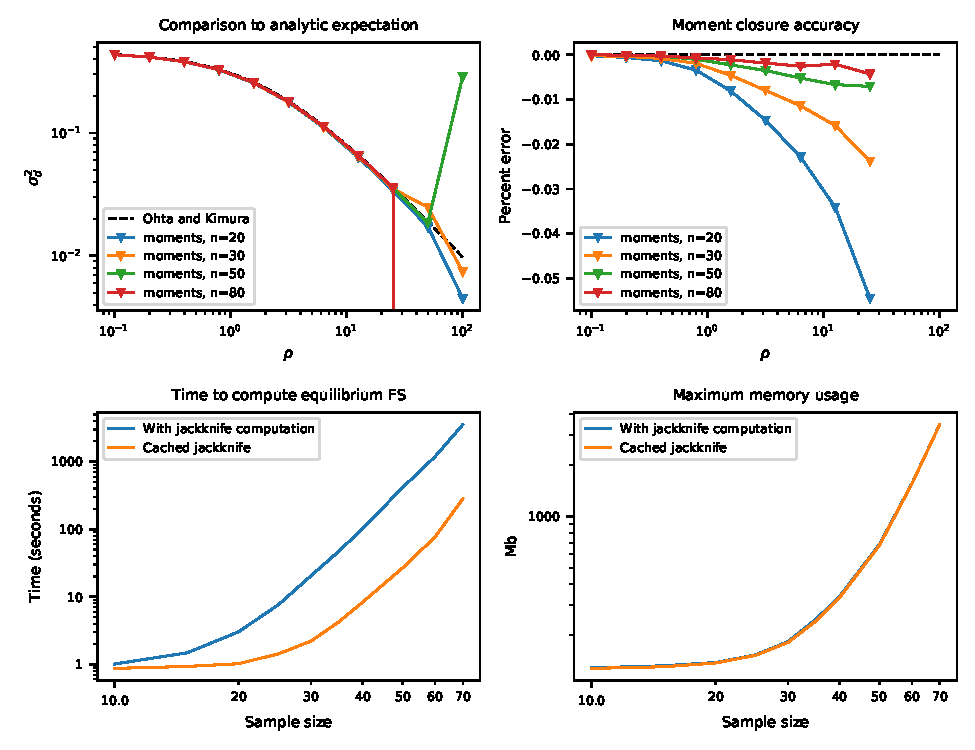
\includegraphics{../figures/jackknife}
    \caption{
        \textbf{Accuracy of the jackknife approximation and runtime} Small
        sample sizes can lead to large error in the moment-closure
        approximation for larger recombination distances or selection
        coefficients. Generally, the jackknife approximation breaks down for
        recombination rates greater than \(\rho\approx30\). While increasing
        sample size leads to more accurate solutions, it comes at the cost of
        both increased runtime and memory usage. Most analyses in this paper
        used sample sizes between 40 and 80.
    }
    \label{fig:jackknife}
\end{figure}

\begin{figure}[ht!]
    \centering
    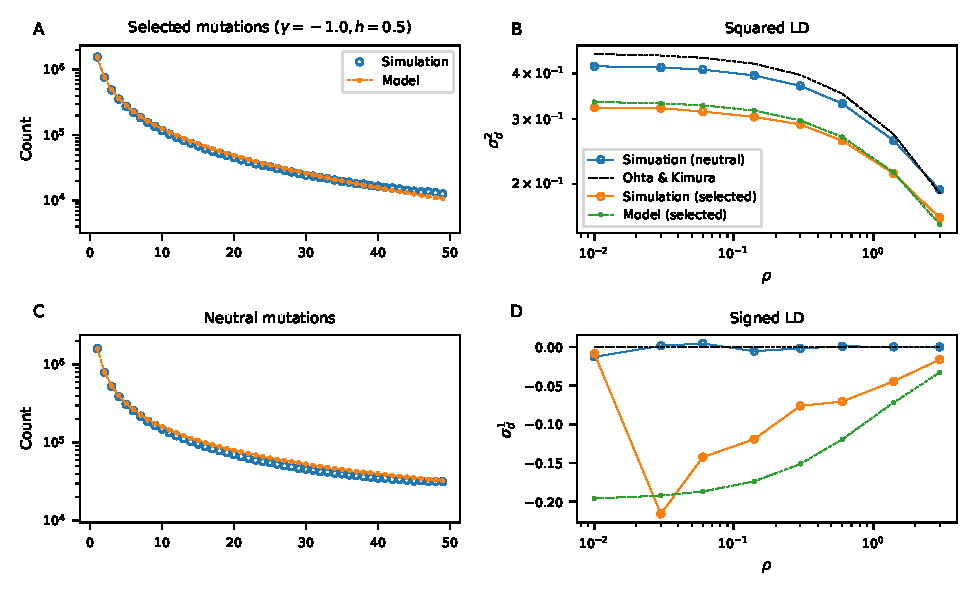
\includegraphics{../figures/bgs_gamma_-1.0_h_0.5_n_50}
    \caption{
        \textbf{Background selection with slightly deleterious mutations.}
        Using an individual based forward simulator
    }
    \label{fig:bgs1}
\end{figure}

\begin{figure}[ht!]
    \centering
    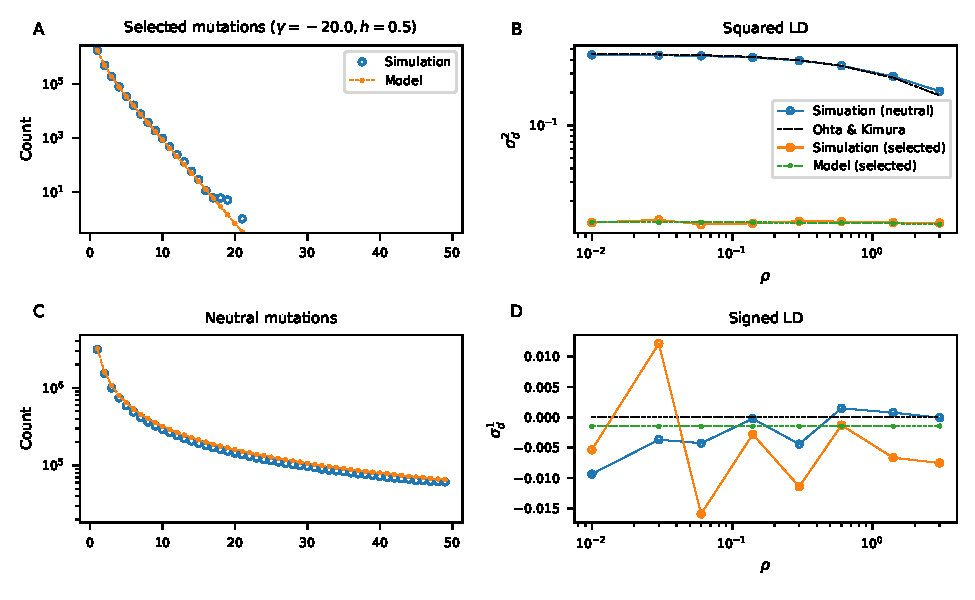
\includegraphics{../figures/bgs_gamma_-20.0_h_0.5_n_50}
    \caption{
        \textbf{Background selection with moderately deleterious mutations.}
    }
    \label{fig:bgs2}
\end{figure}

\begin{figure}[ht!]
    \centering
    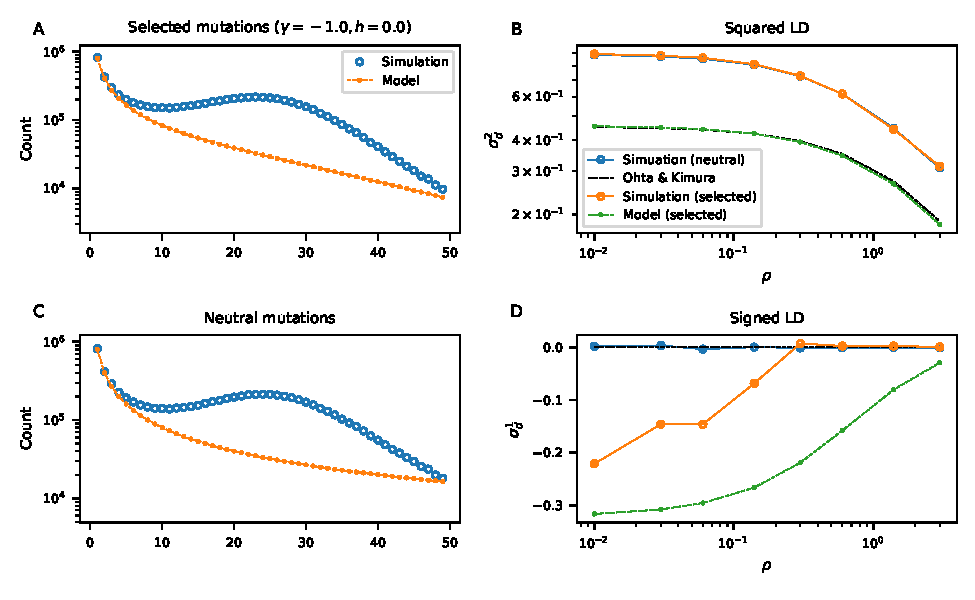
\includegraphics{../figures/bgs_gamma_-1.0_h_0.0_n_50}
    \caption{
        \textbf{Associative overdominance due to slightly deleterious recessive mutations.}
    }
    \label{fig:bgs3}
\end{figure}

\begin{figure}[ht!]
    \centering
    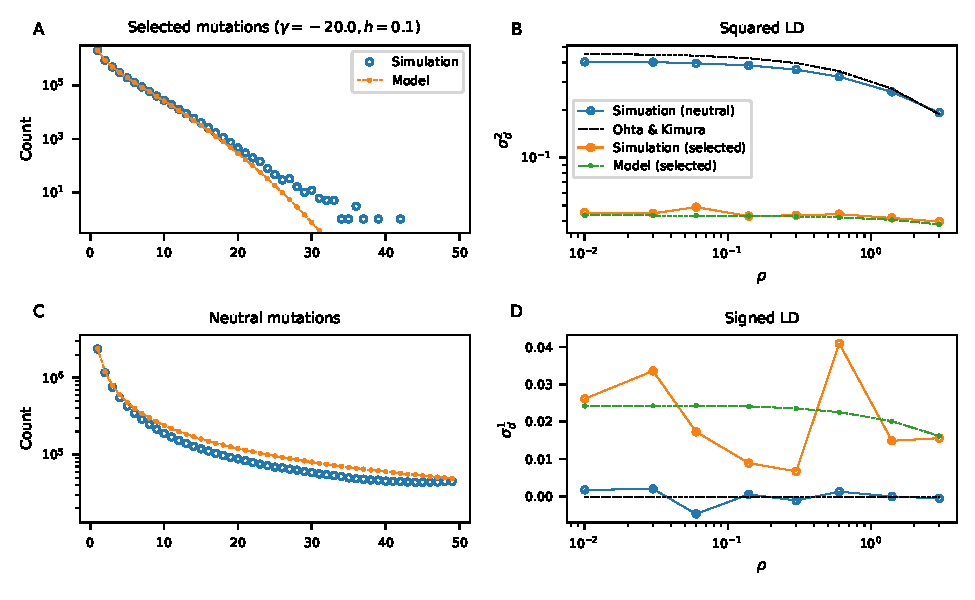
\includegraphics{../figures/bgs_gamma_-20.0_h_0.1_n_80}
    \caption{
        \textbf{Background selection with moderately deleterious recessive mutations.}
    }
    \label{fig:bgs4}
\end{figure}

\begin{figure}[ht!]
    \centering
    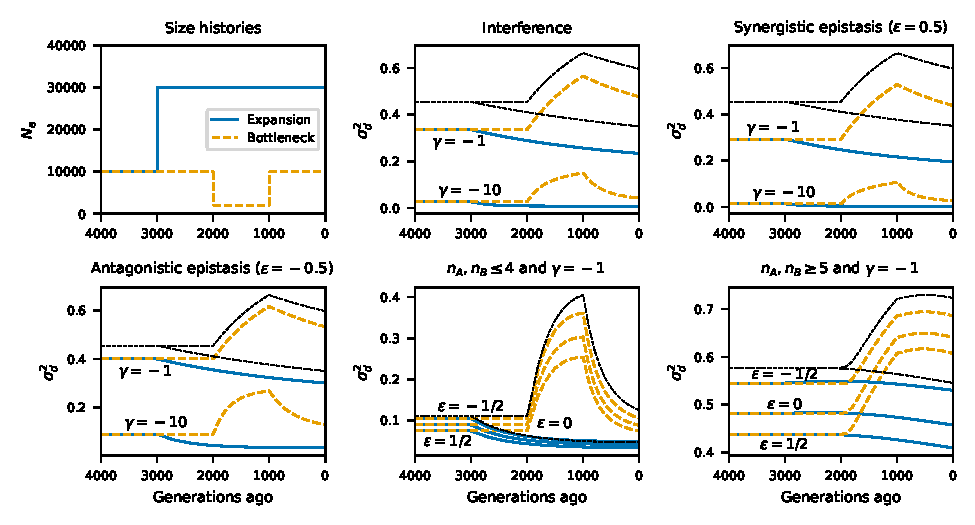
\includegraphics{../figures/demog_bottle_expand.sd2}
    \caption{
        \textbf{.}
    }
    \label{fig:toy_sd2}
\end{figure}

\begin{figure}[ht!]
    \centering
    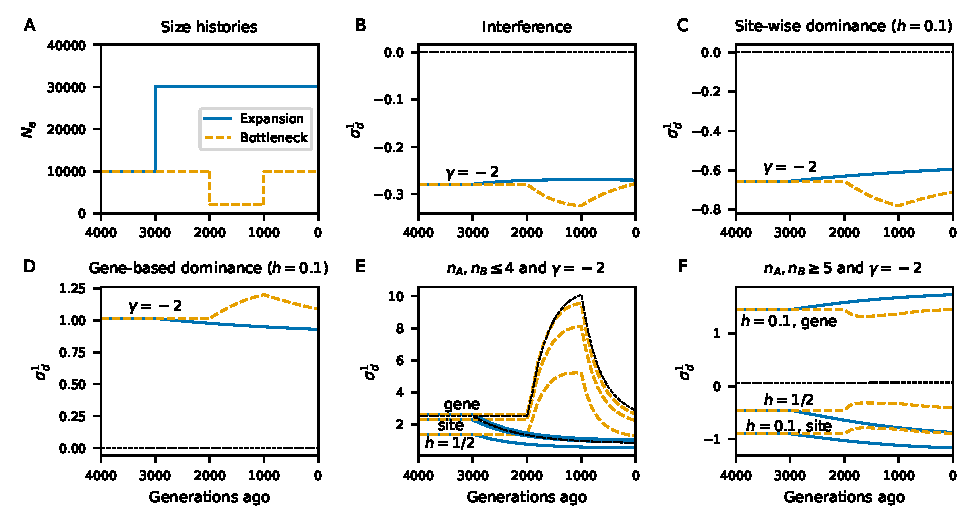
\includegraphics{../figures/demog_bottle_expand.dominance}
    \caption{
        \textbf{.}
    }
    \label{fig:toy_dom}
\end{figure}

\begin{figure}[ht!]
    \centering
    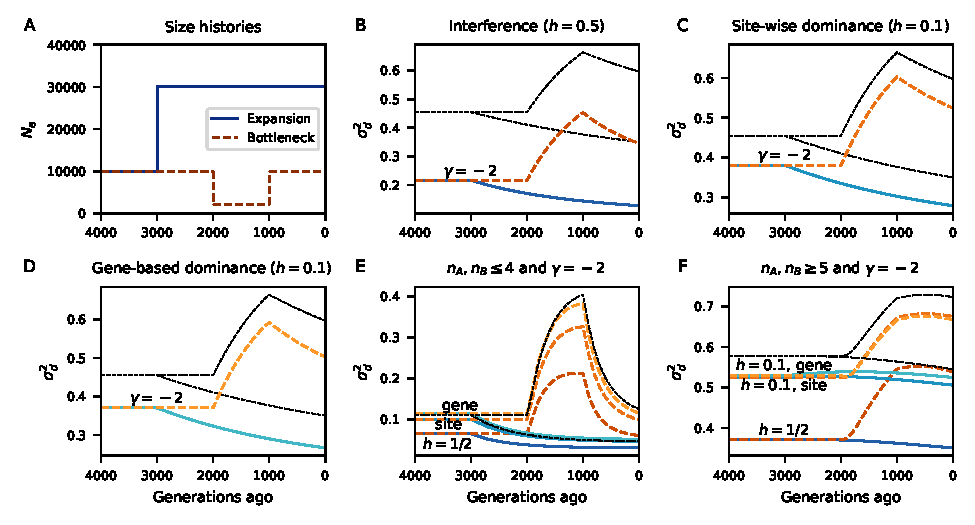
\includegraphics{../figures/demog_bottle_expand.dominance.sd2}
    \caption{
        \textbf{.}
    }
    \label{fig:toy_dom_sd2}
\end{figure}

\begin{figure}[ht!]
    \centering
    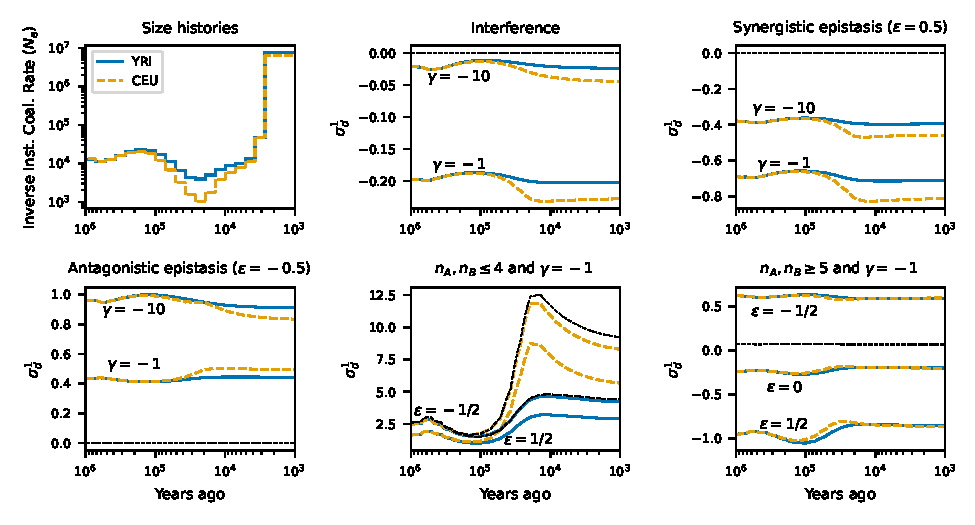
\includegraphics{../figures/demog_YRI_CEU}
    \caption{
        \textbf{.}
    }
    \label{fig:relate}
\end{figure}

\begin{figure}[ht!]
    \centering
    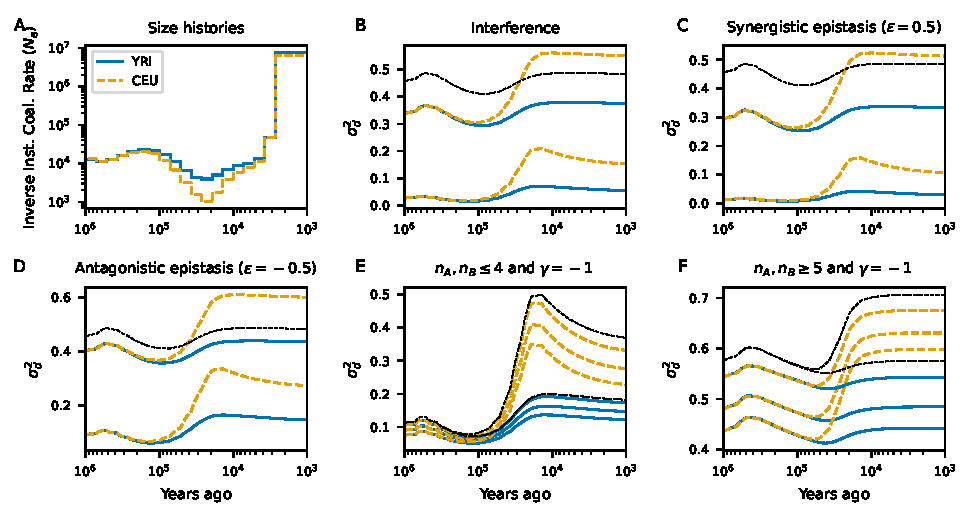
\includegraphics{../figures/demog_YRI_CEU.sd2}
    \caption{
        \textbf{.}
    }
    \label{fig:relate_sd2}
\end{figure}

\begin{figure}[ht!]
    \centering
    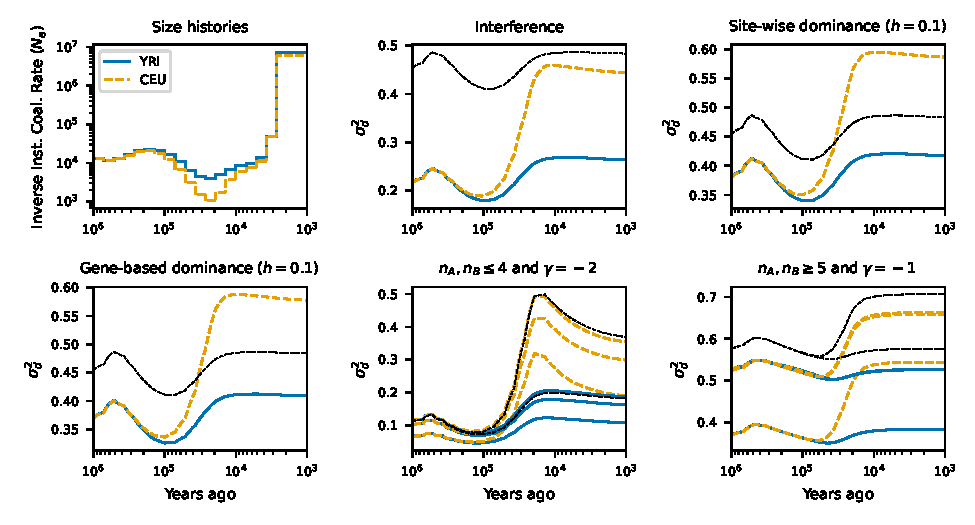
\includegraphics{../figures/demog_YRI_CEU.dominance.sd2}
    \caption{
        \textbf{.}
    }
    \label{fig:relate_dom_sd2}
\end{figure}

\begin{figure}[ht!]
    \centering
    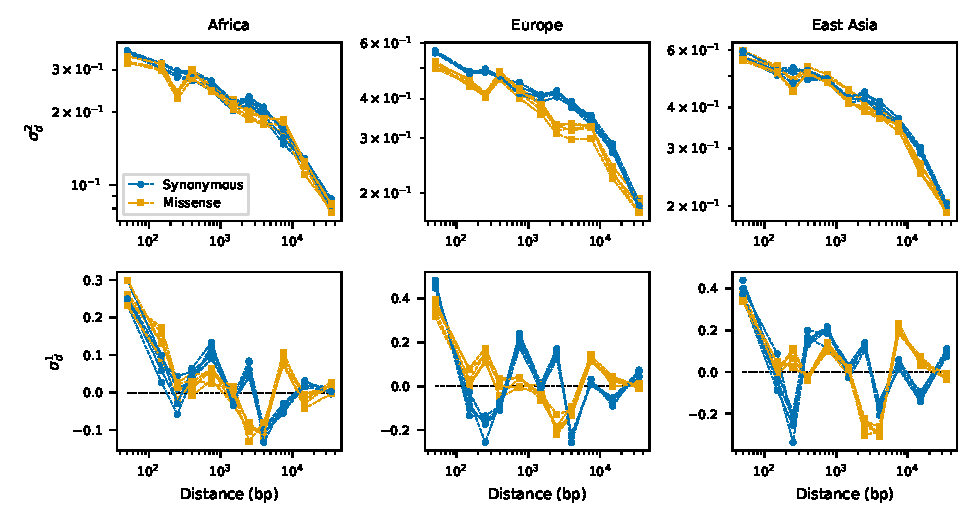
\includegraphics{../figures/ld_decay_gene_wide}
    \caption{
        \textbf{LD decay for pairs of synonymous and missense mutations
        in the same gene.}
    }
    \label{fig:LDgene}
\end{figure}

\begin{figure}[ht!]
    \centering
    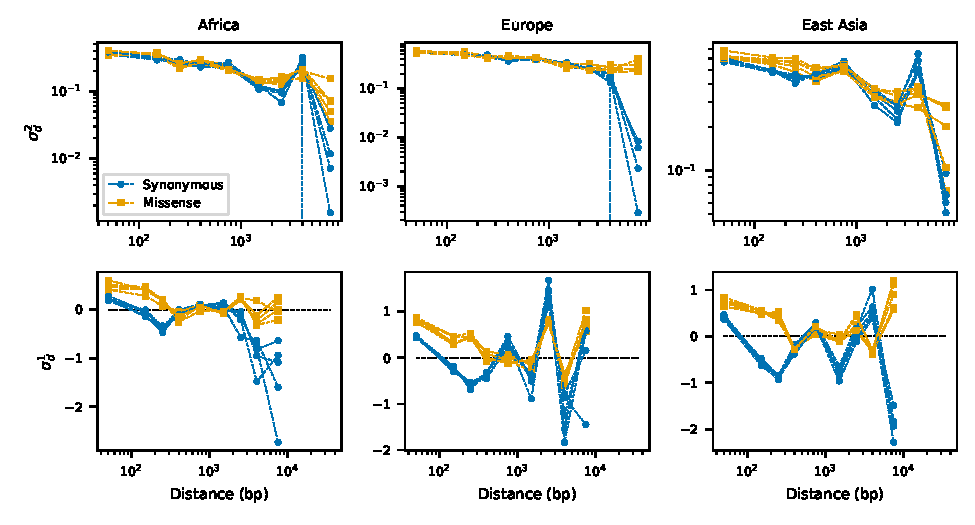
\includegraphics{../figures/ld_decay_in_domain}
    \caption{
        \textbf{LD decay for pairs of synonymous and missense mutations
        that fall inside the same domain.}
    }
    \label{fig:LDwithin}
\end{figure}

\begin{figure}[ht!]
    \centering
    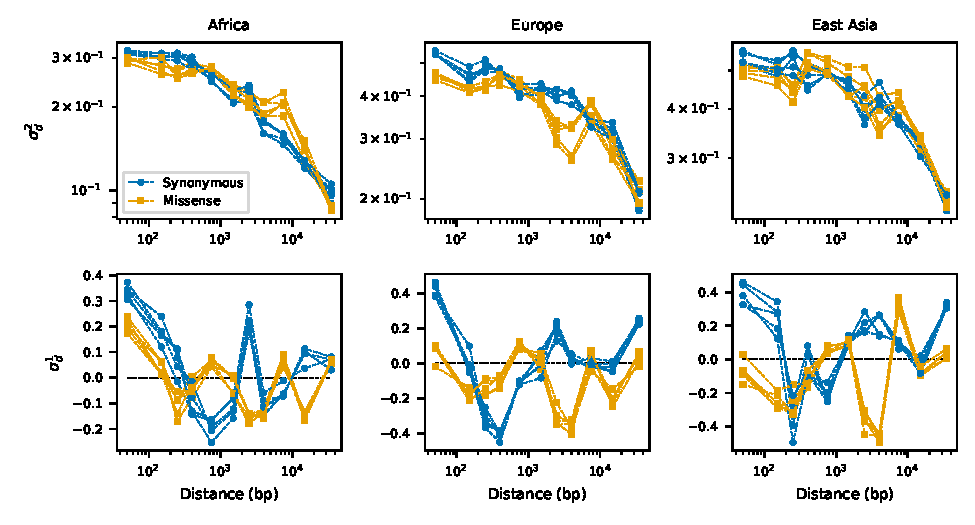
\includegraphics{../figures/ld_decay_outside_domains}
    \caption{
        \textbf{LD decay for pairs of synonymous and missense mutations
        outside of domains.}
    }
    \label{fig:LDoutside}
\end{figure}

\begin{figure}[ht!]
    \centering
    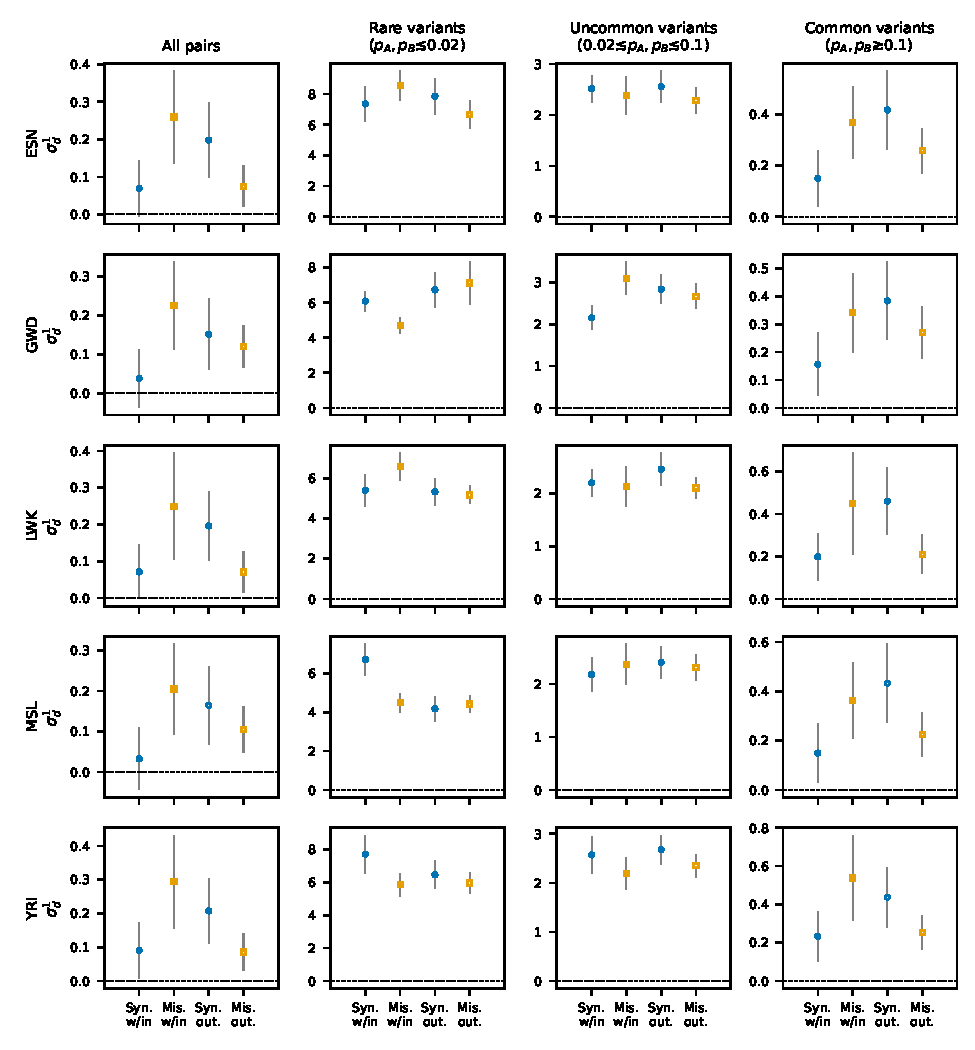
\includegraphics{../figures/data_domains_afr}
    \caption{
        \textbf{LD for pairs of synonymous and missense mutations within the
        same domain and outside domains at matched distances.}
    }
    \label{fig:domainsAFR}
\end{figure}

\begin{figure}[ht!]
    \centering
    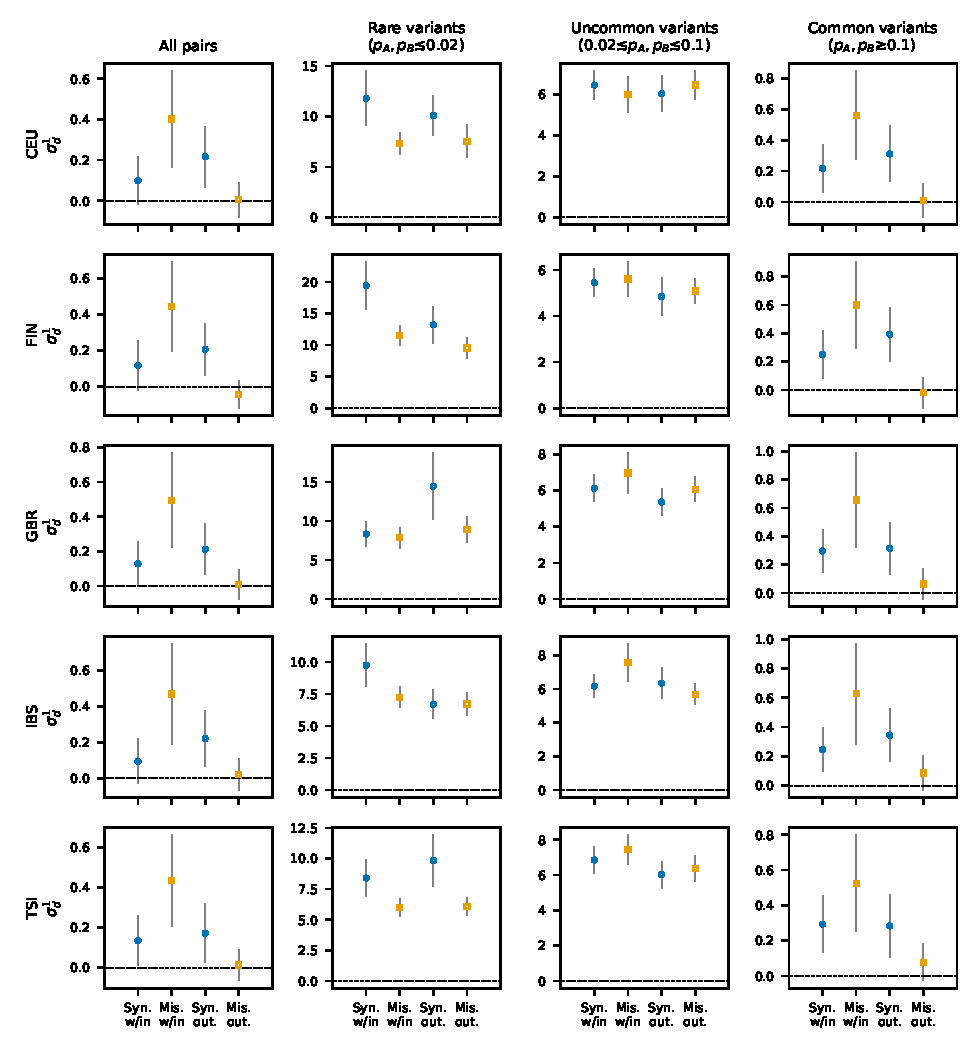
\includegraphics{../figures/data_domains_eur}
    \caption{
        \textbf{LD for pairs of synonymous and missense mutations within the
        same domain and outside domains at matched distances.}
    }
    \label{fig:domainsEUR}
\end{figure}

\begin{figure}[ht!]
    \centering
    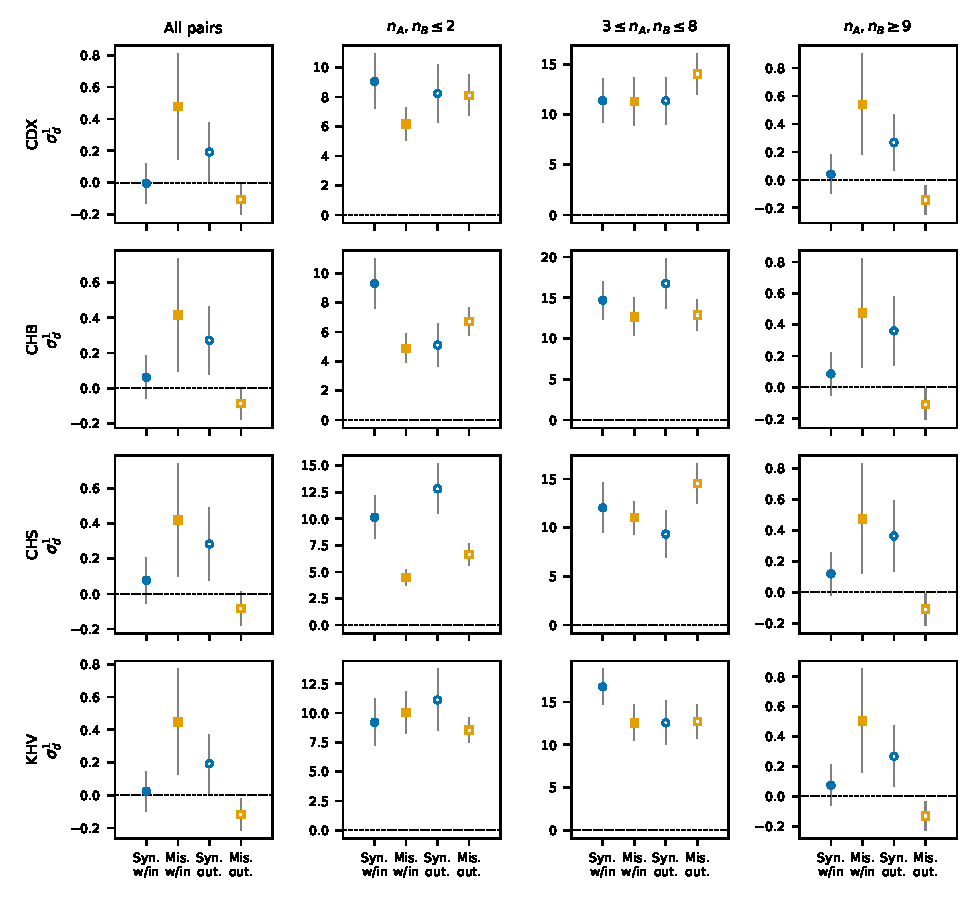
\includegraphics{../figures/data_domains_eas}
    \caption{
        \textbf{LD for pairs of synonymous and missense mutations within the
        same domain and outside domains at matched distances.}
    }
    \label{fig:domainsEAS}
\end{figure}

\begin{figure}[ht!]
    \centering
    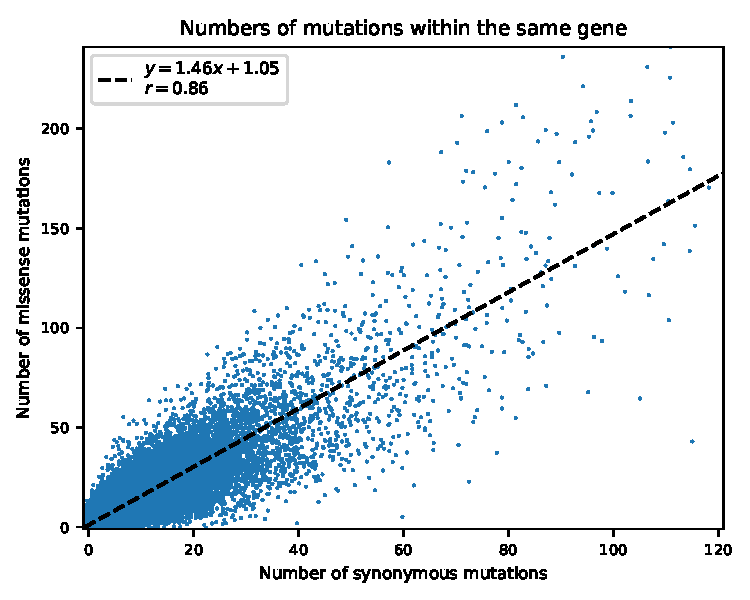
\includegraphics{../figures/mutations_in_genes}
    \caption{
        \textbf{Correlation between numbers of missense and synonymous mutations
        within each gene.}
    }
    \label{fig:mutCorrGene}
\end{figure}

\begin{figure}[ht!]
    \centering
    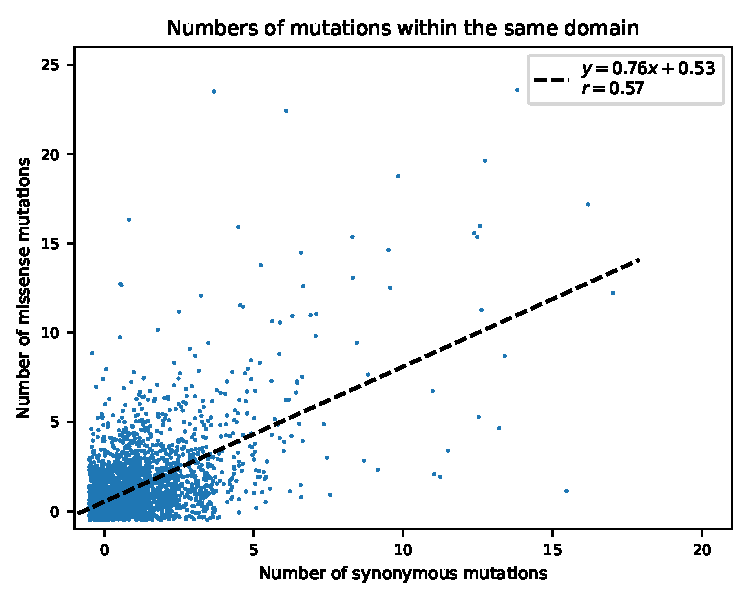
\includegraphics{../figures/mutations_in_domains}
    \caption{
        \textbf{Correlation between numbers of missense and synonymous mutations
        within each annotated domain.}
    }
    \label{fig:mutCorrDomain}
\end{figure}

\begin{figure}[ht!]
    \centering
    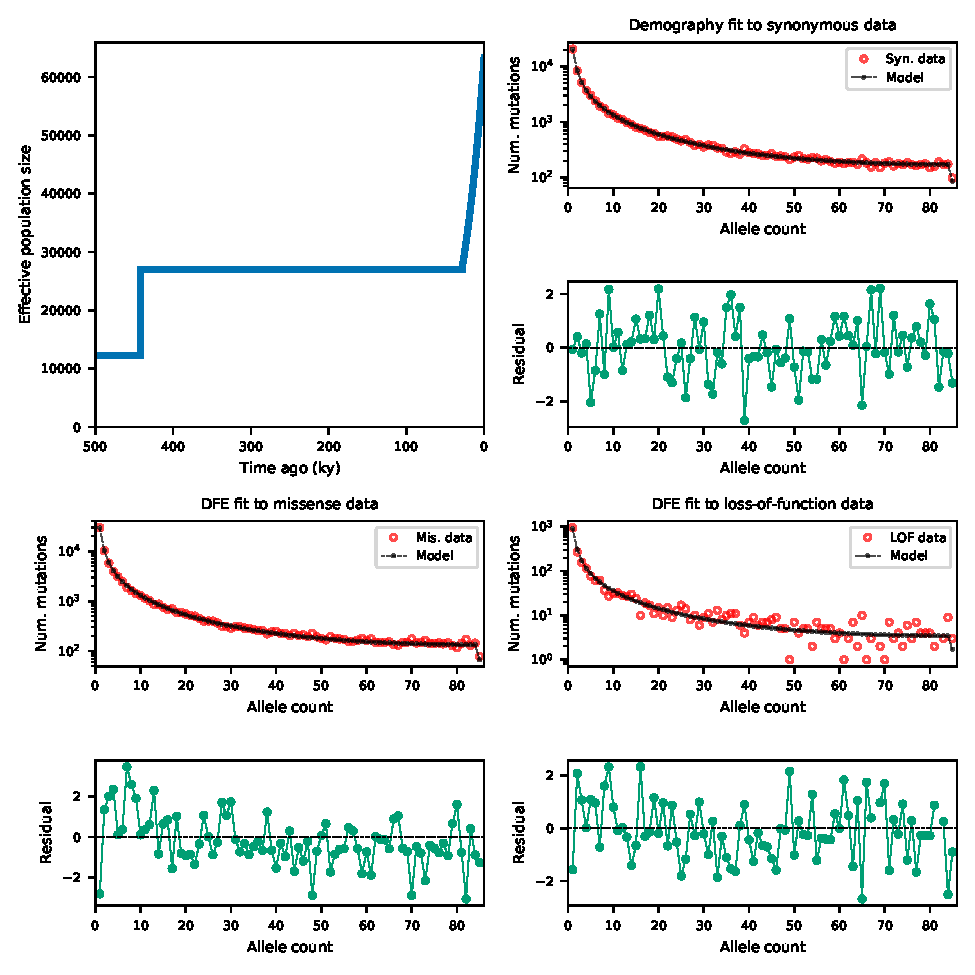
\includegraphics{../figures/msl_demography_dfes}
    \caption{
        \textbf{Demography and DFE for MSL.} A demographic model was fit to
        the folded synonymous SFS, and DFEs were fit to missense and loss-of-function
        SFS. Shown here are DFEs fit with \(h=0.5\). See Table \ref{tab:msldfe} for
        inferred best-fit parameters.
    }
    \label{fig:msldemogdfe}
\end{figure}

\begin{figure}[ht!]
    \centering
    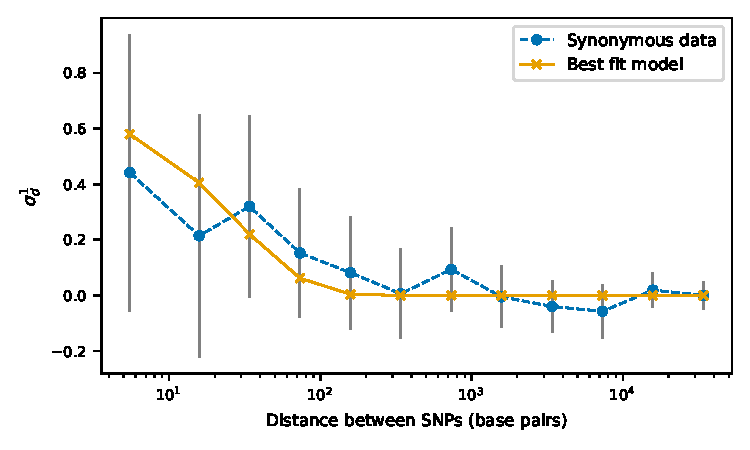
\includegraphics{../figures/msl_mnms}
    \caption{
        \textbf{Optimization of fraction of new mutations arising via
        multinucleotide mutations by distance.} A simple exponential function was fit
        to describe the probability that a pair of mutations arose through a MSM event
        at a given distance \(d\), as \(Ae^{-\lambda d}\). Across all recombination rates
        tested, the best fit parameters were \(A=0.13\) and \(\lambda=0.010\).
    }
    \label{fig:mslmnms}
\end{figure}

\end{document}
